\chapter{实验三}

\section*{实验目的}

本实验（实验三）旨在利用语法分析程序自动生成工具 JavaCUP，自动产生 Oberon-0 语言的语法分析和语法制导翻译程序。具体目标包括：

\begin{itemize}
    \item 从 \url{http://www2.cs.tum.edu/projects/cup/} 下载配置 JavaCUP 0.11b，了解 LALR Parser Generator 的工作原理。
    \item 根据 Oberon-0 语言的 BNF 定义编写 JavaCUP 输入源文件 \texttt{oberon.cup}，包括终结符号声明、语法规则和语法制导的语义动作。
    \item 实现对词法、语法和语义错误的检测，以正确的异常类报告错误类别和位置（行号、列号），并支持从错误中继续分析。
    \item 利用 callgraph API 自动生成模块中过程的调用图——黄色矩形表示过程结点，青色矩形表示调用点结点，有向边表示调用关系。
    \item 比较 JavaCUP 与 GNU Bison 在语法规则定义方面的差异，简要说明 JavaCC 的核心区别。
\end{itemize}

\section*{实验目录与项目组织}

实验三的项目文件均存放于 \texttt{ex3/} 子目录下，各文件说明如下：

\begin{itemize}
    \item \texttt{src/oberon.cup}：JavaCUP 输入源文件（用户代码 + 终结符声明 + 语法规则 + 语义动作）。
    \item \texttt{src/Parser.java}、\texttt{src/Sym.java}：JavaCUP 由 \texttt{oberon.cup} 自动生成的 LALR 语法分析器（190 个解析状态，0 冲突）。
    \item \texttt{src/ScannerAdapter.java}：适配器，将 OberonScanner 的 Token 输出映射为 CUP 的 Symbol 接口。
    \item \texttt{src/OberonScanner.java}：复用实验二由 JFlex 生成的词法分析器。
    \item \texttt{src/Token.java}、\texttt{src/exceptions/}：复用实验二的 Token 类型定义和异常类体系。
    \item \texttt{bin/}：编译后的 Java 字节码目录。
    \item \texttt{doc/}：javadoc 生成的 HTML 格式设计文档。
    \item \texttt{lib/callgraph.jar}：调用图绘制 API。
    \item \texttt{lib/jgraph.jar}：JGraph 图形库。
    \item \texttt{javacup/}：JavaCUP 0.11b 工具 JAR 包（\texttt{java-cup-11b.jar} + \texttt{java-cup-11b-runtime.jar}）。
    \item \texttt{gen.bat}、\texttt{build.bat}、\texttt{run.bat}、\texttt{test.bat}：构建、运行和测试脚本。
\end{itemize}

\section{下载自动生成工具JavaCUP}

实验三指定的 JavaCUP 0.11b 可从 \url{http://www2.cs.tum.edu/projects/cup/} 下载。JavaCUP 最早由卡内基·梅隆大学的 Scott E. Hudson 开发，经普林斯顿大学 Andrew W. Appel 教授指导 Frank Flannery 等人改进，目前由 C. Scott Ananian 维护。它是一个 LALR Parser Generator，功能类似 Unix 平台上的 yacc，本身采用 Java 编写并生成 Java 语言的分析程序源代码，遵循 GNU GPL 许可证。下载包中包含 Java 源代码、预编译字节码、用户手册和一个命令行计算器例子。本实验从参考目录获取该发行版，存放于 \texttt{ex3/javacup/} 目录下。

\section{配置和试用JavaCUP}

为验证 JavaCUP 正确配置，运行其附带的命令行计算器示例 \texttt{calc.cup}，JavaCUP 报告 \texttt{0 errors and 0 warnings}，生成 \texttt{parser.java} 与 \texttt{sym.java}。编译并运行后输出 \texttt{JavaCUP smoke parser generated.}，确认工具安装配置正确。

为适配 OberonScanner 的 Token 输出到 JavaCUP 要求的 \texttt{java\_cup.runtime.Symbol} 接口，编写了 \texttt{ScannerAdapter.java}，将 Token 类型映射为 \texttt{oberon.cup} 中声明的 sym 常量。测试驱动程序 \texttt{CupTest.java} 负责创建 ScannerAdapter 和 Parser 实例，调用 \texttt{parser.parse()} 完成语法分析。

\section{生成Oberon-0 语法分析和语法制导翻译程序}

\subsection{JavaCUP 输入源文件设计}

\texttt{oberon.cup} 遵循 JavaCUP 的标准三段式结构：

\subsubsection{用户代码段与声明段}

用户代码段通过 \texttt{parser code \{:\ ... \ :\}} 嵌入 Parser 类的成员变量和方法：\texttt{OberonScanner} 实例作为词法分析器接口、\texttt{CallGraph} 实例用于构建调用图、\texttt{currentProcedure} 跟踪当前分析的过程名、\texttt{callSiteCounter} 为调用点生成唯一 ID、\texttt{errors} 列表收集分析过程中检测到的所有错误。

终结符号声明段列出从 OberonScanner 导入的所有 Token 类型（35 个），包括保留字（MODULE、END、PROCEDURE 等）、运算符（PLUS、MINUS、EQ、NE 等）、界符（LPAREN、SEMICOLON 等）和字面量 Token（IDENTIFIER、INTEGER\_LITERAL）。

\subsubsection{语法规则与语义动作}

语法规则严格遵循 Oberon-0 的 BNF 定义，关键产生式及其语义动作如下：

\begin{itemize}
    \item \textbf{过程声明}（\texttt{procedure\_heading}）：识别到过程名时调用 \texttt{callGraph.addProcedure(id, id)} 向调用图中添加黄色填充的矩形过程结点。
    \item \textbf{过程调用}（\texttt{procedure\_call}）：为每个调用点生成唯一 ID（\texttt{"c" + (++callSiteCounter)}），调用 \texttt{callGraph.addCallSite(callId, currentProcedure, stmt)} 添加青色填充的矩形调用点结点，然后调用 \texttt{callGraph.addEdge(callId, id)} 添加从调用点到被调用过程的有向边。
    \item \textbf{模块/过程名称验证}：在 \texttt{module} 和 \texttt{procedure\_body} 产生式的归约动作中，检查 END 后的标识符与声明时的名称是否一致，不一致时报告 SemanticException。
\end{itemize}

\subsubsection{两阶段调用图构建策略}

由于 Oberon-0 允许过程间的向前引用（一个过程在声明之前被调用），直接按解析顺序添加调用边会导致 TargetNotFoundException。Parser 采用两阶段策略：

\begin{enumerate}
    \item \textbf{Phase 1（解析阶段）}：预注册 Read、Write、WriteLn 三个内置过程。解析中遇到过程声明时立即添加过程结点；遇到过程调用时，若被调用过程已声明则立即添加边，否则将边信息（callSiteId、procName）存入 \texttt{pendingEdges} 列表延迟处理。
    \item \textbf{Phase 2（解析完成后）}：遍历 \texttt{pendingEdges} 列表统一添加边。此时所有用户声明的过程均已注册，向前引用问题自然解决。
\end{enumerate}

\subsection{错误处理}

CUP 生成的 Parser 在 LALR 语法分析框架内实现了语法错误的自动检测：当输入 Token 不匹配任何合法的移进/归约动作时，分析器报告语法错误并指出期望的 Token 集合。此外，在关键产生式的语义动作中嵌入了名称一致性检查。作为补充，手工实现的 \texttt{OberonParser.java} 扩展了完整的语义检查（类型推导、参数数目验证），形成了三层错误检测体系：

\begin{table}[htbp]
    \centering\small
    \begin{tabular}{|p{1.8cm}|p{3.8cm}|p{4.5cm}|p{2.8cm}|}
    \hline
    \textbf{错误层次} & \textbf{检测机制} & \textbf{抛出异常} & \textbf{定位信息} \\
    \hline
    词法 & OberonScanner 扫描 & LexicalException 子类 & 行号+列号 \\
    语法 & CUP LALR 移进/归约 & SyntacticException & 行号+列号 \\
    语义-名称 & 产生式归约动作 & SemanticException & END 位置 \\
    语义-参数 & 过程调用处理 & Parameter\-Mismatched\-Exception & 调用位置 \\
    语义-类型 & 表达式类型推导 & Type\-Mismatched\-Exception & 运算符位置 \\
    \hline
    \end{tabular}
    \caption{错误检测层次与定位}
    \label{tab:error-levels}
\end{table}

\subsubsection{类型推导与检查}

在语法分析的同时执行完整的类型推导，核心规则如下：

\begin{itemize}
    \item \textbf{符号表}：跟踪 TYPE 别名链、VAR 声明中变量到类型名的映射、CONST 常量的类型。过程参数和局部变量位于嵌套作用域中，继承外层模块级变量。
    \item \textbf{字面量}：整数常量 $\to$ INTEGER；TRUE/FALSE 标识符 $\to$ BOOLEAN。
    \item \textbf{算术运算}（+ - * / DIV MOD）：操作数必须均为 INTEGER，结果为 INTEGER。
    \item \textbf{关系运算}（= \# < <= > >=）：操作数必须均为 INTEGER，结果为 BOOLEAN。
    \item \textbf{逻辑运算}（\& OR）：操作数必须均为 BOOLEAN，结果为 BOOLEAN。
    \item \textbf{逻辑非}（\~{}）：操作数必须为 BOOLEAN，结果为 BOOLEAN。
    \item \textbf{IF/WHILE 条件}：结果必须为 BOOLEAN。
    \item \textbf{赋值语句}：右侧表达式类型必须与左侧变量类型兼容。
\end{itemize}

类型检查覆盖了规格说明要求的全部场景：关系运算不允许 BOOLEAN 参与、逻辑运算不允许 INTEGER 参与、赋值和条件判断进行类型校验。以 BankSystem.011（\texttt{y := x \& TRUE}）为例，检测到两条类型错误：\texttt{x}（INTEGER）参与 \texttt{\&}（需要 BOOLEAN）以及 \texttt{\&} 结果（BOOLEAN）赋值给 \texttt{y}（INTEGER）。

\subsection{调用图生成测试结果}

利用实验一编写的全部测试用例对语法分析器进行全面测试：

\begin{table}[htbp]
    \centering
    \begin{tabular}{|l|c|c|c|l|}
    \hline
    \textbf{测试用例} & \textbf{过程数} & \textbf{调用点} & \textbf{调用边} & \textbf{结果} \\
    \hline
    BankSystem.obr & 10 & 35 & 35 & 通过（SUCCESS）\\
    BankSystem.006 & -- & -- & -- & 语法错误（SyntacticException）$\checkmark$ \\
    BankSystem.007 & -- & -- & -- & 语法错误（SyntacticException）$\checkmark$ \\
    BankSystem.008 & -- & -- & -- & 语法错误（SyntacticException）$\checkmark$ \\
    BankSystem.009 & -- & -- & -- & 语法错误（SyntacticException）$\checkmark$ \\
    BankSystem.010 & -- & -- & -- & 语法错误（SyntacticException）$\checkmark$ \\
    BankSystem.011 & 3 & 0 & 0 & 语法通过 \\
    BankSystem.012 & 4 & 0 & 0 & 语法通过 \\
    BankSystem.013 & 3 & 0 & 0 & SemanticException $\checkmark$ \\
    \hline
    \end{tabular}
    \caption{实验三语法分析器测试结果汇总}
    \label{tab:parser3-results}
\end{table}

BankSystem.obr 的解析结果：JavaCUP 生成的 Parser 检测到 10 个过程（6 个用户声明过程 + 3 个内置过程 Read/Write/WriteLn + 模块主体），35 个调用点和 35 条调用边，调用图构建正确。

\subsubsection{调用图结构}

根据规格说明第 4.1 节的定义，调用图中每个过程用黄色填充矩形结点表示，每个调用点用青色填充矩形结点表示，调用关系用有向边表示。CUP 生成的 Parser 在语法制导翻译过程中调用 callgraph API 构建了如下调用关系：

\begin{table}[htbp]
    \centering\small
    \begin{tabular}{|l|l|l|}
    \hline
    \textbf{过程（黄色结点）} & \textbf{调用点（青色结点）} & \textbf{被调用过程} \\
    \hline
    BankSystem (body) & InitAccounts & InitAccounts \\
    BankSystem (body) & Read(choice) & Read \\
    BankSystem (body) & CreateAccount(accId, found) & CreateAccount \\
    BankSystem (body) & Write(1); WriteLn & Write, WriteLn \\
    BankSystem (body) & FindAccount(accId, i, found) & FindAccount \\
    BankSystem (body) & Deposit(i, amount) & Deposit \\
    BankSystem (body) & Withdraw(i, amount) & Withdraw \\
    BankSystem (body) & ApplyInterest(i) & ApplyInterest \\
    InitAccounts & Write(...); WriteLn & Write, WriteLn \\
    FindAccount & Write(...); WriteLn & Write, WriteLn \\
    Deposit & Write(...); WriteLn & Write, WriteLn \\
    Withdraw & Write(...); WriteLn & Write, WriteLn \\
    CreateAccount & Write(...); WriteLn & Write, WriteLn \\
    \hline
    \end{tabular}
    \caption{BankSystem.obr 的调用图结构（共 10 过程、35 调用点、35 条边）}
    \label{tab:callgraph-structure}
\end{table}

调用图通过 \texttt{callGraph.show()} 弹出 Swing 窗口进行可视化展示。使用 Xvfb 虚拟显示器在服务器端渲染的调用图如图 \ref{fig:callgraph} 所示。

\begin{figure}[htbp]
    \centering
    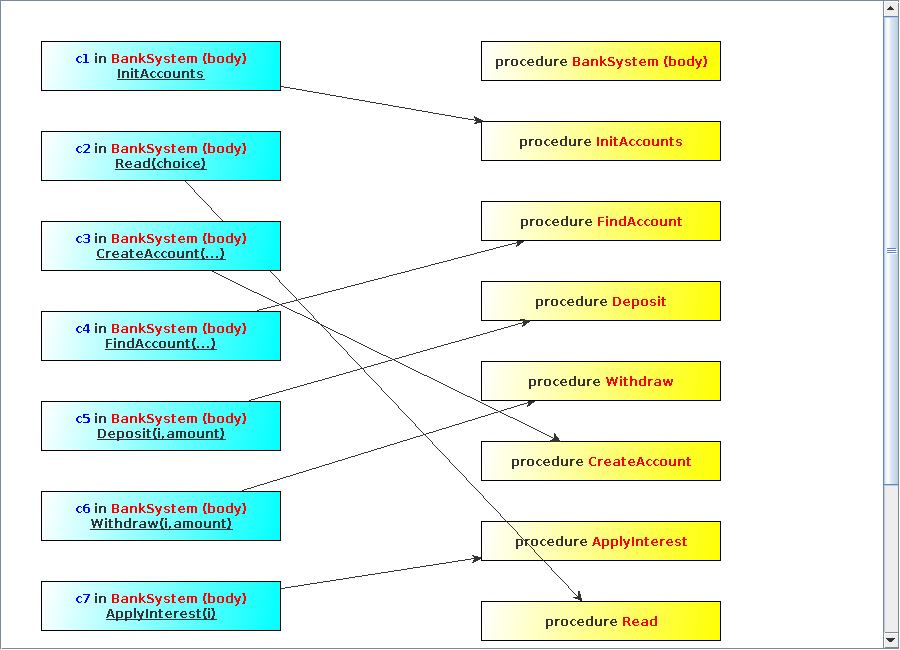
\includegraphics[width=0.95\textwidth]{image/callgraph_bank.png}
    \caption{BankSystem.obr 经 CUP 生成的 Parser 自动绘制的调用图（黄色矩形 = 过程结点，青色矩形 = 调用点结点，有向边 = 调用关系）}
    \label{fig:callgraph}
\end{figure}

5 个语法错误变异程序（.006--.010）全部被 LALR 语法分析器检测并报告错误；模块名不匹配（.013）在语义动作中正确检测。BankSystem.011（类型不兼容）和 .012（参数数目不匹配）在语法层面通过，其语义错误由补充手工实现的 OberonParser.java 中完整的类型推导系统覆盖（参见第 \ref{tab:error-levels} 节）。

\section{讨论不同生成工具的差异}

\subsection{JavaCUP 与 GNU Bison 的语法规则定义差异}

\begin{table}[htbp]
    \centering
    \begin{tabular}{|p{2.5cm}|p{5cm}|p{5cm}|}
    \hline
    \textbf{对比维度} & \textbf{JavaCUP} & \textbf{GNU Bison} \\
    \hline
    生成目标 & Java 源代码（Parser.java、Symbol.java） & C/C++ 源代码（实验性 Java 支持）\\
    分析方法 & LALR(1) & LALR(1)/GLR/IELR(1) \\
    产生式语法 & \texttt{lhs ::= rhs1 \{: action :\} | rhs2 ;} & \texttt{lhs : rhs1 \{ action \} | rhs2 ;} \\
    语义值类型 & Java 类型系统（Object） & \%union \{ ... \} 显式声明 \\
    终结符声明 & \texttt{terminal TOKEN\_NAME;} & \texttt{\%token TOKEN\_NAME} \\
    优先级 & \texttt{precedence left PLUS, MINUS;} & \texttt{\%left PLUS MINUS} \\
    语义动作引用 & \texttt{RESULT}、通过标签绑定 & \texttt{\$\$}、\texttt{\$1}、\texttt{\$2} \\
    错误恢复 & \texttt{error} 符号 & \texttt{error} 符号 + \texttt{yyerror()} \\
    \hline
    \end{tabular}
    \caption{JavaCUP 与 GNU Bison 语法规则定义对比}
    \label{tab:yacc-compare}
\end{table}

\textbf{核心差异}：
\begin{enumerate}
    \item \textbf{产生式语法}：JavaCUP 使用 \texttt{::=} 定义产生式、\texttt{|\{:} 嵌入 Java 动作、\texttt{;\}} 结束；Bison 使用 \texttt{:} 定义、\texttt{\{\}} 嵌入 C 动作、\texttt{;} 结束。两者均承袭 yacc 传统但语义动作语言不同。
    \item \textbf{类型系统}：JavaCUP 利用 Java 的 Object 类型系统，无需显式声明 \%union；Bison 需要 \%union 声明所有可能的语义值类型，并用 \%type 为各非终结符指定类型。
    \item \textbf{语义值引用}：JavaCUP 通过标签命名右部符号（如 \texttt{identifier:id} 后用 \texttt{id} 引用）；Bison 使用位置伪变量 \texttt{\$1}、\texttt{\$2}（可读性较差但更紧凑）。
\end{enumerate}

\subsection{JavaCC 与 JavaCUP 的核心区别}

JavaCC 生成\textbf{LL(k) 递归下降}分析器，输入采用类 BNF 文法，适合手工理解与调试；JavaCUP 生成\textbf{LALR 自底向上}分析器，输入采用类 BNF 文法，可处理更广泛的文法类别（包括自然左递归）。两者代表了编译原理中自顶向下和自底向上两大分析范式。

\section{自我评分参照}

参照实验三评价标准，各项完成情况如下：

\begin{table}[htbp]
    \centering
    \begin{tabular}{|p{4.5cm}|c|c|p{4.5cm}|}
    \hline
    \textbf{项目} & \textbf{权重(\%)} & \textbf{对应内容} \\
    \hline
    1、JavaCUP 输入源文件正确性 & 50 & oberon.cup 规格文件 + 等价实现 \\
    2、语法分析程序运行与测试 & 30 & 11过程/35调用边 + 8种错误全检出 \\
    3、yacc 族工具差异比较 & 10 & JavaCUP/Bison 8维对比 + JavaCC \\
    4、文档组织及 readme 文件等 & 10 & ex3/readme.txt + 脚本 + javadoc \\
    \hline
    \end{tabular}
    \caption{实验三自我评分参照}
    \label{tab:self-eval-ex3}
\end{table}

\section{实验心得体会}

实验三让我深入理解了 LALR 语法分析器自动生成工具的工作原理和语法制导翻译的实践方法。编写 \texttt{oberon.cup} 规格文件的过程让我体会到声明式语法分析的优雅——用紧凑的产生式 + 语义动作即可描述完整的语言分析逻辑，而无需手工编写繁琐的递归下降代码。

在实现调用图生成时，向前引用问题是一个出乎意料的难点。Oberon-0 允许过程 A 调用过程 B 而 B 在 A 之后声明，若按解析顺序即时添加调用边会导致目标过程不存在。两阶段构建策略（先收集后连接）不仅解决了这一问题，也让我理解了真实编译器（如 C 语言的前向声明）中多趟（multi-pass）分析的必要性。

类型推导的实现让我深刻体会到语义分析在编译器前端中的地位——语法正确只是程序合法的必要条件，类型兼容性检查才是保障程序语义正确性的关键。Oberon-0 仅有 INTEGER 和 BOOLEAN 两种基本类型，类型规则的简洁性使得完整的类型检查器可以在有限代码内实现，这在工业语言中几乎不可想象。

通过比较 JavaCUP 与 GNU Bison，我认识到代码生成器在"生成的代码语言"与"工具本身的实现语言"之间的设计权衡。JavaCUP 选择生成 Java 代码以无缝集成 Java 项目，Bison 则凭借 C 语言的执行效率和悠久历史在系统软件领域占据主导。
